\chapter{Состав и структура компонента технического зрения и обоснование выбора технических и программных средств} \label{chapt4}

\section{Обзор и обоснование выбора программных средств} \label{sect4_1}

Проектирование СТЗ уже давно превратилось в широко распространённую техническую отрасль, предоставляющую решения любой направленности и любой сложности исполнения. Не в последнюю очередь это следствие развития программных пакетов и библиотек, предоставляющих доступ к использованию базовых функций технического зрения. В настоящее время существует множество программных пакетов, ориентированных на разработку в различных средах программирования и операционных системах. Какие-то из них развиваются с использованием открытого исходного кода и являются бесплатными к использованию, но при этом ничуть не уступают в функционале мощному платному ПО. Для создания простых СТЗ уже не нужно обладать углублёнными навыками программирования, хотя всё ещё остаётся огромный пласт знаний, обязательных для проектировщика: устройство и работа СТЗ, структуры данных, форматы видеосигналов и многое другое. Помимо этого, остро стоит и выбор языка программирования, поскольку разные языки имеют разную направленность в проектах.

Среди базовых библиотек начального уровня можно выделить три пакета для языка Python: NumPy, SciPy и Matplotlib. Все они появились достаточно давно --- несколько лет назад --- и до сих пор получают развитие и обновления; все они в разной мере являются обязательными при использовании более продвинутых решений для создания СТЗ. NumPy ориентирован на быструю работу с многомерными массивами данных, что широко применяется в работе с цветными изображениями, также он предоставляет базовые функции для работы с кадрами, такие как размытие, повышения резкости, контрастности и прочее. SciPy выполняет инженерные расчёты с векторами и матрицами, к примеру, анализ сигналов. Matplotlib предоставляет возможности работы с двумерными и трёхмерными графиками и диаграммами, в том числе, с гистограммами и их анализом. Также среди библиотек начального уровня можно упомянуть пакет Pillow, не слишком продвинутый, но содержащий базовые функции для работы с изображениями.

Пакет OpenCV уже целенаправленно разрабатывается для работы с техническим зрением и с 2006 года накопил в себе широкий набор функций, которые делают данное решение своего рода стандартом в проектировании СТЗ. Это достигается ещё и за счёт того, что OpenCV не скован одним языком программирования, а доступен для практически всех распространённых языков, таких, как C/C++, Java, Matlab, Lua и других.Его самым большим недостатком можно считать низкую скорость работы с большими объёмами данных, что может быть компенсировано другими библиотеками под этот язык, например, NumPy для языка Python. Пакет имеет очень хорошую документированность и большое число литературы и сетевых ресурсов. Кроме того, OpenCV является бесплатным для использования и распространяется по лицензии BSD.

В среде фреймворка .NET тоже существуют свои решения, например, AForge.NET. Этот пакет не столь мощный и всеобъемлющий, как OpenCV, но тоже достаточно функцонален. Поддерживается только один язык --- C\#, на котором и написан. Является также бесплатным к использованию по лицензии GPL. Существует также ещё один проект, своего рода надстройка над AForge.NET под названием Accord.NET, расширяющая его функционал, а с 2015 года распространяющаяся в составе AForge.NET.

Ещё одним пакетом программ для среды .NET можно назвать SimpleCV, который, однако, не предоставляет широких возможностей для работы и слабо подходит для сложных задач. К тому же, слабая документированность и не очень активное комьюнити сказываются на его популярности среди разработчиков.

Что касается сложных программных комплексов, то можно упомянуть программный пакет LabView, предоставляющее функции по работе с системами сбора и обработки данных. Техническое зрение является лишь частью функционала данного ПО. Разработка программ осуществляется на собственном языке программирования G. Однако, данное ПО является платным и имеет закрытый исходный код, кроме того, его функционал на платформах, отличных от Microsoft Windows, является ограниченным.

В эту же категорию попадает и MatLab, который также является платным ПО с закрытым исходным кодом, но практически незаменим в вопросах обработки изображений, посколькую включает в себя множество подпрограмм для разных областей работы. Язык программирования также свой собственный, интерпретируемый, под названием MATLAB.

Сейчас техническое зрение тесно связано с технологиями машинного обучения, поскольку задача распознавания лежит в том числе и в области нейросетевого подхода. В первую очередь тут стоит упомянуть TensorFlow от Google. Данный пакет бесплатен к использованию и широко применяется в задачах машинного обучения, однако, работа в ней требует наличия у инженера базовых знаний работы с нейронными сетями. Она достаточно требовательна к ресурсам компьютера или смартфона, на котором запускается, однако, умеет эффективно использовать ресурсы графического процессора. Тем не менее, сейчас, когда рынок графических процессоров переживает кризис, и цены на оборудование сильно взлетели, использование TensorFlow в любительских проектах является менее целесообразным.

Также можно упомянуть ПО для глубокого машинного обучения CatBoost от компании <<Яндекс>>. Он основан не на нейронных сетях, а на так называемом <<градиентном бустинге>> и имеет открытый исходный код. Также поддерживает работу с GPU.

Помимо уже перечисленных, можно упомянуть программные пакеты меньшего масштаба. Например, в среде iOS существует основанная на OpenGL библиотека GPUImage. В среде Android можно использовать BoofCV, которая имеет хорошо оптимизированные алгоритмы и целиком написана на Java. В проектах с роботизацией существует пакет ROS (Robot Operating System), а для параллельных вычисления можно задействовать архитектуру CUDA от NVidia.

Таким образом, можно отметить, что рынок предлагает множество программных пакетов, ориентированных на самые разные задачи и условия разработки СТЗ. Особенно широкий набор библиотек доступен разработчикам Python и C++, самых широко применяемых языков программирования на сегодняшний день.

\section{Обоснование выбора технических средств} \label{sect4_2}

\section{Описание структуры модуля машинного зрения} \label{sect4_3}

\section{Анализ результатов работы} \label{sect4_4}

\subsection{Анализ быстродействия} \label{sect4_4_1}

\subsection{Работа с поверхностями} \label{sect4_4_2}

Помимо базовых задач, выполняемых интегрированной в станок СТЗ, существуют ещё и расширенные задачи, реализуемые с помощью дополнительных модулей вспомогательного типа. Они были перечислены в подразделе \cref{ssect3_3_3}, однако, в случае с конкретным видом используемого оборудования важно понимать его возможности при работе с разными типами изделий. Поскольку описываемая в разделе \cref{sect1_5} модульная установка с ЧПУ является устройством широкого применения, могут встречаться обрабатываемые изделия с разными свойствами поверхностей металлических, полимерных и комбинированных деталей. Так, модуль глубины изображения, ответственный за построение трёхмерных сцен в кадре, показал наличие проблем в отображением определённого рода поверхностей, что ограничивает его применение в рамках платформы с ЧПУ.

Основной проблемой при выборе оборудования является его зачастую недостаточно подробная документация и, чем сложнее устройство оборудования, тем больше его характеристик можно выяснить лишь опытным путём. В документации используемой камеры нет чётких данных, с какими из поверхностей её работа является полноценной и достоверной. Данный модуль глубин не является мультиспектральным, т.~е., лазерная сетка имеет лишь одну длину волны излучения --- 850 нм, что относится к ИК-диапазону. Также производителем заявляется общая погрешность измерения, равная 1~\% на 1 метр. Таким образом, можно составить список материалов, на которых стоит проверить работу датчика глубин, сопоставить процент ошибки измерения с конкретными параметрами их свойств и выявить ограничения использования такого оборудования.

\begin{figure}[ht]
	\centerfloat{
		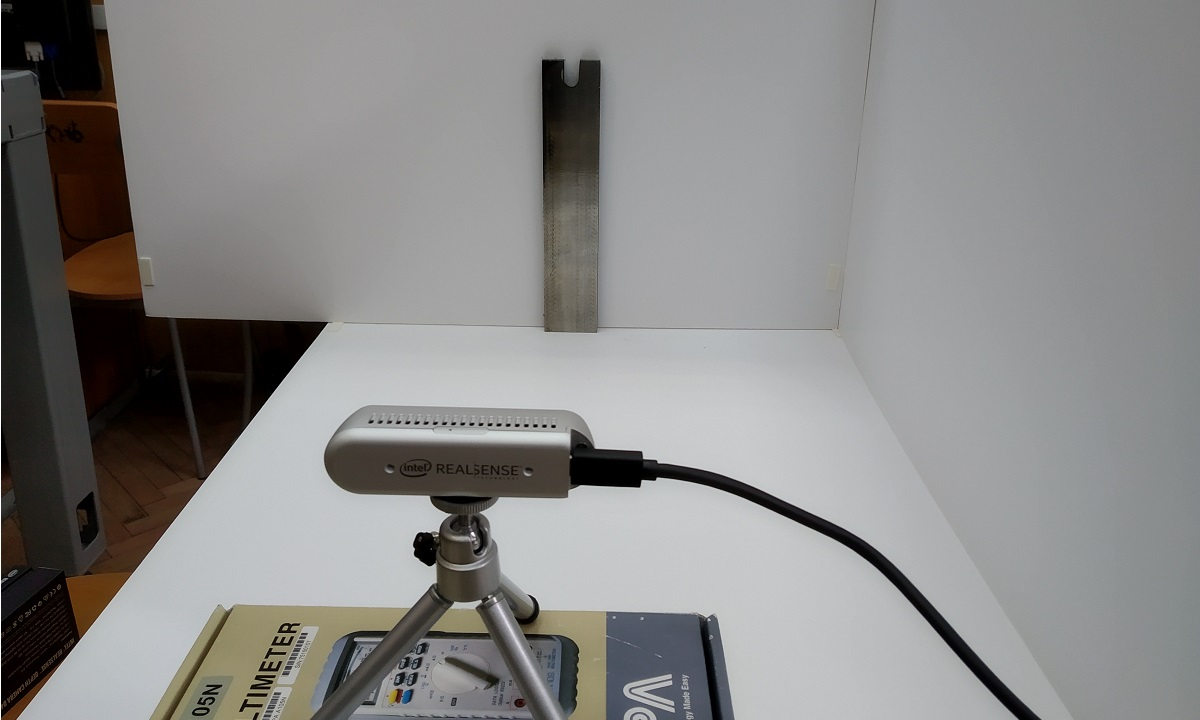
\includegraphics[width=15cm]{images/izmer.jpg}
	}
	\caption{Условия проведения тестов модуля глубин}\label{fig:izmer}
\end{figure}

Образцы с указанными характеристиками размещались на рабочем расстоянии от камеры (750 мм), освещение естественное (дневной свет) и люминесцентные лампы (рис. \cref{fig:izmer}). Проверялись две характеристики образца: средний процент ошибки на 50 измерений и видимость объекта в построенной сцене. Средний процент ошибки рассчитывается по формуле \cref{eq_4_1}:

\begin{equation}
\Delta d = \frac {\max_{n} [\overline{d} - d_i]} {\overline{d}} \cdot 100 \%,
\label{eq_4_1}
\end{equation}

где $\overline{d}$ --- среднее значение расстояния на 50 измерений, $d_i$ --- текущее значение расстояния в этом измерении, $n$ --- количествоизмерений для обного образца, $n = 50$.

Видимость объекта в кадре оценивалась по визуальным характеристикам построенной сцены. В частности, проверялась ситуация, когда лазерный луч не мог быть отражён от каких-то участков объекта по причине особых свойств поверхности, в результате чего измерение в данной области считалось некорректно и игнорировалась при построении, т. е., область имела вид провала на объекте. Также некорректность построения может выражаться в мерцании областей и неровностей там, где предполагается плоская поверхность. Таким образом, полная видимость означает, что объект в кадре виден целиком, без разрывов и искажений, а его вид неизменен в течение всего времени тестирования конкретного образца. Частичная видимость свидетельствует о наличии вышеперечисленных проблем с отображением по отдельности или совокупно, но при этом форма объекта всё ещё определяется в сцене. Отсутствующая видимость подразумевает, что объект в кадре не распознаётся, нельзя чётко указать его форму. 

Список рассмотренных поверхностей представляет собой, по большей части, распространённые конструкционные материалы с разным типом обработки и, соответственно, параметром шероховатости поверхности. К ним были добавлены пластик (полипропилен), текстолит, зеркало обычное с амальгамным покрытием и зеркало молибденовое как пример поверхности с эталонным параметром шероховатости. В качестве базового показателя качества поверхности используется параметр шероховатости Rz, представляющий собой сумму средних значений высот 5 наибольших выступов профиля и глубин 5 наибольших впадин профиля в пределах некоторой базовой длины поверхности. Все рассмотренные поверхности представлены в таблице \cref{tab:tp2}:

\begingroup
\centering
\captionsetup[table]{skip=7pt} % смещение положения подписи
\begin{longtable}[c]{|p{5cm}|p{3.5cm}|c|c|p{3cm}|}
	\caption{Перечень образцов}\label{tab:tp2}
	\\[-0.45\onelineskip]
	\hline
	Материал & Вид обработки & Rz & Ошибка, \% & Видимость \tabularnewline \hline
	Сталь 45\footnote{ГОСТ 1050-2013} & Шлифование & 10--80 & 0,1 & Полная \tabularnewline \hline
	--- & Растачивание & 80 & 0,22 & Полная \tabularnewline \hline
	--- & Фрезерование & 40 & 0,21 & Полная \tabularnewline \hline
	--- & Доводка & 2 & 1,67 & Полная \tabularnewline \hline
	Чугун СЧ-15\footnote{ГОСТ 1412-85} & Растачивание & 80 & 0,21 & Полная \tabularnewline \hline
	--- & Фрезерование & 40 & 0,22 & Полная \tabularnewline \hline
	Бронза БрАЖ9-4\footnote{ГОСТ 18175-78} & Шлифование & 10--80 & 0,25 & Полная \tabularnewline \hline
	--- & Растачивание & 80 & 0,24 & Полная \tabularnewline \hline
	--- & Фрезерование & 40 & 0,26 & Полная \tabularnewline \hline
	Алюминий Д16Т\footnote{ГОСТ 4784-97} & Хим. Окс. Э\footnote{Покрытие химическое оксидированное электропроводное} & 2,5 & 1,8 & Частичная \tabularnewline \hline
	Полипропилен\footnote{ГОСТ 26996-86} & --- & 160 & 0,94 & Полная \tabularnewline \hline
	Текстолит\footnote{ГОСТ 2910-74} & --- & 40 & 7 & Полная \tabularnewline \hline
	Зеркало бытовое & --- & 0,5 & 7,2 & Частичная \tabularnewline \hline
	Зеркало молибденовое & --- & 0,15 & 100 & Отсутствует \tabularnewline \hline
\end{longtable}
\endgroup

Процент ошибки для каждого образца замерядся в ПО Depth Quatity Tool от Intel RealSense. Полученные данные для металлических поверхностей можно привести в виде графика (рис. \cref{fig:plot-rz}):

\begin{figure}[ht]
	\centerfloat{
		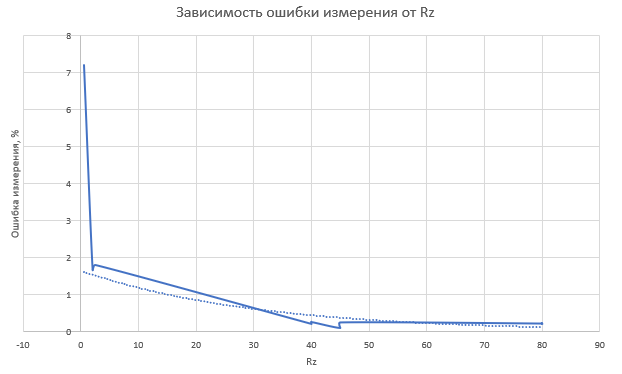
\includegraphics[width=15cm]{images/plot_rz.png}
	}
	\caption{График зависимости процента ошибки от показателя шероховатости поверхности Rz}\label{fig:plot-rz}
\end{figure}

Из данного графика можно отметить скачкообразное падение точности измерения при достижении некоторого значения параметра Rz. Ввиду малого количества образцов точное значение выделить сложно, однако, если провести линию тренда на таком графике, то получим примерный показатель Rz, равный 15 мкм. Поверхности чище этого показателя будут выходить за пределы паспортной точности, а значит, что использование вспомогательных устройств данного типа будет неэффективным и при работе с такими поверхностями необходимо измерение иным оборудованием. Тем не менее, используемый модуль глубины успешно справляется с подавляющим большинством поверхностей, как металлических, так и неметаллических, и показывает процент ошибки сильно ниже паспортного, в пределах 0,3~\%.

\section{Выводы по четвертой главе} \label{sect4_5}